% % % % % % % % % % % % % % % % % % % % % % % % % % % % % % % % % % % % % % % % % % % %
%                                                                                     %
% Short Sectioned Assignment LaTeX Template Version 1.0 (5/5/12)                      %
% This template has been downloaded from: http://www.LaTeXTemplates.com               %
%                                                                                     %
% Original author:  Frits Wenneker (http://www.howtotex.com)                          %
%                                                                                     %
% Modified by: Fco Javier Sueza Rodríguez (fcosueza@disroot.org)                      %
%                                                                                     %
% Changes:                                                                            %
%	    - Custom Chapters, Sections and Subsections (titlesec package)                %
%           - Document type scrbook (oneside)                                         %
%           - Use babel-lang-spanish package and marvosym                             %
%           - Use hyperref, enumitem, tcolorbox and glossaries packages               %
%           - Use Time New Roman (mathptmx), Helvetic and Courier fonts               %
%                                                                                     %
% License: CC BY-NC-SA 3.0 (http://creativecommons.org/licenses/by-nc-sa/3.0/)        %
%                                                                                     %
% % % % % % % % % % % % % % % % % % % % % % % % % % % % % % % % % % % % % % % % % % % %

%-----------------------------------------------%
%	              Packages                  %
%-----------------------------------------------%

\documentclass[paper=a4, fontsize=11pt, oneside]{scrbook}

% ---- Text Input/Output ----- %

\usepackage[T1]{fontenc}
\usepackage[utf8]{inputenc}
\usepackage{mathptmx}
\usepackage[scaled=.92]{helvet}
\usepackage{courier}
\usepackage[indent=12pt]{parskip}

\usepackage{geometry}
\geometry{verbose,tmargin=3cm,bmargin=3cm,lmargin=2.6cm,rmargin=2.6cm}

% ---- Language ----- %

\usepackage[spanish]{babel}
\usepackage{marvosym}

% ---- Another packages ---- %

\usepackage{amsmath,amsfonts,amsthm}
\usepackage{graphics,graphicx}
\usepackage{titlesec}
\usepackage{fancyhdr}
\usepackage{tcolorbox}
\usepackage{hyperref}
\usepackage{enumitem}
\usepackage[automake]{glossaries}

%--------------------------------------------------------------------%
%                      Customizing Document                          %
%--------------------------------------------------------------------%


% ----------- Custom Chapters, Sections and Subsections -------------- %

\titleformat{\chapter}[display]
			{\bfseries\Huge}
			{Tema \ \thechapter} {0.5ex}
			{\vspace{1ex}\centering}

\titleformat{\section}[hang]
			{\bfseries\Large}
			{\thesection}{0.5em}{}

\titleformat{\subsection}[hang]
			{\bfseries\large}
			{\thesubsection}{0.5em}{}

\titleformat{\subsubsection}[hang]
			{\bfseries\large}
			{\thesubsubsection}{0.5em}{}

\hypersetup{
    colorlinks=true,
    linkcolor=black,
    urlcolor=magenta
}

% ------------------- Custom heaaders and footers ------------------- %

\pagestyle{fancyplain}

\fancyhead[]{}
\fancyfoot[L]{}
\fancyfoot[C]{}
\fancyfoot[R]{\thepage}

\renewcommand{\headrulewidth}{0pt} % Remove header underlines
\renewcommand{\footrulewidth}{0pt} % Remove footer underlines

\setlength{\headheight}{13.6pt} % Customize the height of the header

% --------- Numbering equations, figures and tables ----------------- %

\numberwithin{equation}{section} % Number equations within sections
\numberwithin{figure}{section} % Number figures within sections
\numberwithin{table}{section} % Number tables within sections

% ------------------------ New Commands ----------------------------- %

\newcommand{\horrule}[1]{\rule{\linewidth}{#1}} % Create horizontal rule command


%----------------------------------------------------------------------------------------
%	TÍTULO Y DATOS DEL ALUMNO
%----------------------------------------------------------------------------------------

\title{
\vspace{10ex}
\normalfont \normalsize
\Huge \textbf{Tarea 7: Instalación y Configuración de Ubuntu Desktop 22.04 LTS}
}
\author{Francisco Javier Sueza Rodríguez}
\date{\normalsize\today}

%----------------------------------------------------------------------------------------
%                                     DOCUMENTO
%----------------------------------------------------------------------------------------
\begin{document}

\maketitle

\thispagestyle{empty}

\vspace{68ex}

\begin{center}
    \begin{tabular}{l l}
        \textbf{Centro}: & IES Aguadulce \\
        \textbf{Ciclo Formativo}: & Desarrollo Aplicaciones Web (Distancia)\\
        \textbf{Asignatura}: & Sistemas Informáticos\\
        \textbf{Tema}: & Tema 7 -  Instalación y Configuración de Linux\\
    \end{tabular}
\end{center}

\newpage

\tableofcontents

\newpage

\listoffigures

\newpage

\section{Caso Práctico}
Uno de los directivos de la empresa ha solicitado a Ada la puesta en marcha de un sistema operativo GNU/LINUX en su equipo y ésta traslada la petición a Antonio para que lo haga conjuntamente con Juan. Ellos fueron los que instalaron en los equipos Windows 10 y Windows 8.1, y ahora instalarán el nuevo sistema operativo en una partición libre que dejaron en su momento, precisamente porque pensaron que en un futuro podrían recibir peticiones de este tipo.

\section{Actividades}
\subsection{Actividad 1: Un poco de documentación}
\subsubsection{Enunciado}
Indica lo que permiten o no permiten las siguientes licencias de derechos de autor Creative Commons. Rellena la siguiente tabla atendiendo al ejemplo de la primera fila.

\begin{figure}[H]
    \centering
    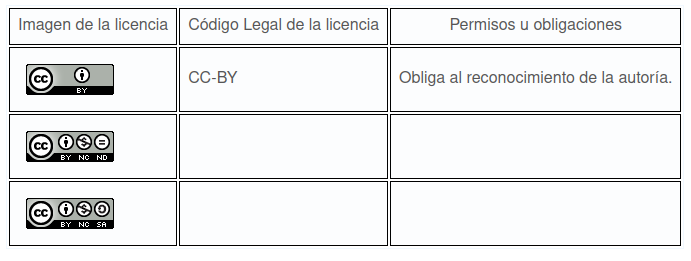
\includegraphics[scale=0.60]{tabla-cc.png}
    \caption{Tabla de licencias Creative Commons}
\end{figure}

Responde a las siguientes preguntas:

\begin{enumerate}[label=\alph*.]
    \item ¿Cuál es el principal objetivo de la licencia GNU GPL?
    \item ¿Qué podemos hacer con un software cuya licencia cumpla la libertad 3?
    \item Si tengo un software cuya licencia cumple la libertad 1: ¿Podemos distribuir copias? Razona la respuesta.
\end{enumerate}

\subsubsection{Solución}
En primer lugar, vamos a rellenar la tabla sobre las licencias Creative Commons especificando el código legal de cada una y sus permisos u obligaciones.

En la siguiente figura, se muestra la tabla completada.

\begin{figure}[H]
    \centering
    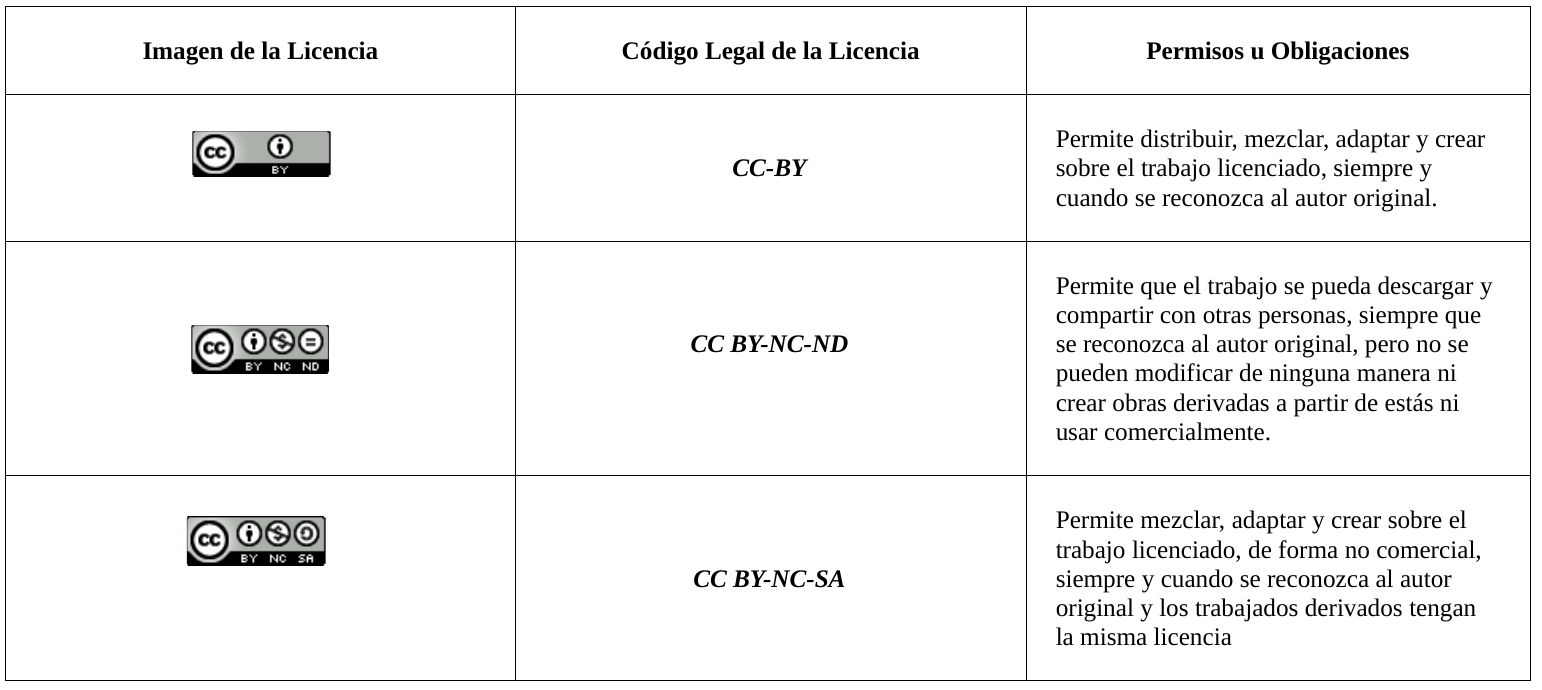
\includegraphics[scale=0.40]{tabla-cc-completa.png}
    \caption{Tabla licencias Creative Commons - Completada}
\end{figure}

A continuación, vamos a \textbf{responder a las preguntas} planteadas sobre la licencia GPL:

\begin{enumerate}[label=\alph*.]
    \item El \textbf{principal objetivo} de la licencia GPL es el de garantizar la libertad para modificar y compartir el software que se encuentre bajo dicha licencia y sus derivados.

    \item Con un software cuya licencia cumpla la \textbf{libertad 3}, podremos realizar todas las \textbf{modificaciones} que consideremos oportunas en dicho software y \textbf{redistribuirlo}.

    \item Si tenemos un software que cuya licencia \textbf{sólo} cumple la \textbf{libertad 1} no tenemos permisos para redistribuirlo, ya que esta libertad solo otorga permisos para \textbf{adaptarlo a nuestra necesidades} y \textbf{estudiar su funcionamiento}, quedando excluido en este punto la redistribución.

    Para que el software se pudiera redistribuir libremente debería cumplir la \textbf{libertad 3}.
\end{enumerate}

\subsection{Actividad 2: Instalación de Ubuntu}

\textbf{¡IMPORTANTE!} Si estás utilizando Oracle VirtualBox como software de virtualización para estas tareas, es posible que cuando instales Ubuntu 22.04 y lo inicies no veas nada en la pantalla (pantalla negra). Para evitar/arreglar esto, con la VM apagada prueba a cambiar en su configuración lo siguiente: ``Configuración > Pantalla > Controlador gráfico: VMSVGA''

\subsubsection{Enunciado}
Instala la versión 22.04 LTS del sistema operativo Ubuntu (versión Desktop) en la partición libre que dejaste en la máquina virtual de la tarea 4. Esta versión está disponible sólo para sistemas de 64 bits, en caso de tener que instalar una versión para 32 bits lee las indicaciones del apartado 2.- Información de interés. Es muy importante recordar que se deben mantener las instalaciones de Windows de las tareas previas.

Si no realizaste la tarea 4, para que ésta sea válida tienes que instalar Ubuntu Desktop 22.04 LTS junto con Windows 10 en una máquina virtual definida con un tamaño de disco duro de 70 GB y con dos particiones de 35 GB, una para cada sistema. En ese caso primero debes instalar Windows 10 y luego Ubuntu Desktop  22.04 LTS.

Durante la instalación de Ubuntu debes definir un usuario local cuyo nombre de usuario sea la primera letra de tu nombre seguido de tus apellidos completos, por ejemplo, para \textbf{José Luis Pérez Puertas} el usuario debería ser \textbf{jlperezpuertas}. Respecto a la clave de este usuario ponle \textbf{admin2223}.

\textbf{Capturas}:
\begin{itemize}
    \item Elección del archivo de instalación del sistema.
    \item Inicio del proceso de instalación.
    \item Actualizaciones y otro software. Justifica las opciones elegidas.
    \item Tipo de instalación: ``Instalar Ubuntu junto a Windows 10'', ``Borrar disco e instalar Ubuntu''' o ``Más opciones''. Justifica tu elección.
    \item Creación del usuario y establecimiento de la contraseña.
    \item Muestra de que el sistema ha sido debidamente instalado.
\end{itemize}

\subsubsection{Solución}
En este ejercicio vamos a realizar la instalación de \textbf{Ubuntu 22.04 LTS} (\textbf{Jammy Jellyfish}), la última versión estable de la distribución de Canonical lanzada en Abril de 2022.

Para realizar la instalación, vamos a llevar a cabo una \textbf{serie de pasos} que enumeraremos a continuación, ilustrándolos con las capturas de pantalla pedidas de forma que el proceso se entienda más claramente.



% Bibliography

%\newpage
%\bibliography{citas}
%\bibliographystyle{unsrt}

\end{document}